\hypertarget{ux6df1ux5ea6ux5b66ux4e60ux57faux7840ux7406ux8bba}{%
\chapter{深度学习基础理论}\label{ux6df1ux5ea6ux5b66ux4e60ux57faux7840ux7406ux8bba}}

\hypertarget{ux673aux5668ux5b66ux4e60ux7684ux5206ux7c7b}{%
\section{机器学习的分类}\label{ux673aux5668ux5b66ux4e60ux7684ux5206ux7c7b}}

在人工智能领域，``学习''这个词（即``机器学习''，Machine Learning）有特定的含义。它不是指死记硬背，而是指模型从数据中自动寻找规律的能力。具体可分为以下三种：

\hypertarget{ux4e00ux76d1ux7763ux5b66ux4e60ux8ddfux7740ux6807ux51c6ux7b54ux6848ux5b66}{%
\subsection{一、监督学习：跟着``标准答案''学}\label{ux4e00ux76d1ux7763ux5b66ux4e60ux8ddfux7740ux6807ux51c6ux7b54ux6848ux5b66}}

这是最常见、也最容易理解的学习方式。

核心思想：我们给模型提供一大堆已经``标好答案''的数据（称为``有标签的数据集''），然后要求模型给出的输出尽可能接近这个``标准答案''。

通俗比喻：使用《参考答案》。你（模型）在做一道练习题（输入数据，比如一张图片），然后你立刻翻到书后面对一下答案（标签，比如``这是一只猫''）。你做的题越多，就越能总结出``猫''的特征（比如有尖耳朵、胡须）。下次再看到一张没有答案的猫图片时，你也能认出它来。

实际应用：

图像分类：你给AI看了数百万张标有``狗''、``汽车''、``人脸''的图片，它最终学会了区分它们。

AlphaFold2：这是一个著名的生物模型。科学家们给它输入蛋白质的``序列''（练习题），并告诉它在``蛋白质数据库(PDB)''中对应的``3D结构''（标准答案）。最终，它学会了预测新序列的3D结构。

\hypertarget{ux4e8cux65e0ux76d1ux7763ux5b66ux4e60ux81eaux5df1ux627eux89c4ux5f8bux5b66}{%
\subsection{二、无监督学习：自己``找规律''学}\label{ux4e8cux65e0ux76d1ux7763ux5b66ux4e60ux81eaux5df1ux627eux89c4ux5f8bux5b66}}

这种方式更有挑战性，也更接近人类的自主探索。

核心思想：我们只给模型一大堆``没有答案''的数据，让模型自己去发现数据中隐藏的结构或规律。（这也包括了``自监督学习''，即模型自己给自己创造``答案''）。

通俗比喻：整理一堆杂乱的拼图，想象有人给了你一大箱混杂的拼图碎片（无标签数据），但没有给你参考的成品图。你（模型）的任务不是拼出某个``正确''的图案，而是自己去发现规律。比如，你可能会把所有``蓝色天空''的碎片放在一起，把``红色屋顶''的碎片放在一起。你虽然不知道最终拼出的是什么，但你理解了碎片之间的``相似性''。

实际应用（及分支）：

扩散模型：想象一张清晰的照片。你（模型）先学习一个``加噪声''的过程，即如何一步步把照片变得完全模糊。然后，你再学习这个过程的``逆向操作''：如何从一张充满噪声的、模糊的图片开始，一步步``去噪''，最终还原出清晰的图像。

为什么是无监督？这个过程中，你唯一需要的就是大量清晰图片，而不需要人工告诉它``这是猫''或``这是狗''。

大语言模型自回归：这就是大规模的``完形填空''。模型阅读了互联网上所有的文本（无标签数据），它的任务就是预测下一个词。比如，看到``今天天气很\_\_''，它通过学习海量文本，知道后面接``好''的概率最高。它自己从上下文中创造了``标签''。

VAE（变分自编码器）：这像一个高明的``速记画家''。它先把一张复杂的图像（输入）``压缩''成几个关键特征（编码），然后再尝试用这几个特征把原画``复原''出来（解码）。它的``评分标准''有两部分：1. 复原的画和原画有多像？2. 你的压缩方式是不是足够简洁且符合某种规律（如高斯分布）？

对比学习：核心思想是``物以类聚''，学习一个特征空间，在其中相似的数据点（称为~``正样本对''）应该靠得很近，不相似的数据点（称为~``负样本对''）应该离得很远。通过对同一个数据点（如一张图片）施加不同的数据增强（如随机裁剪、随机颜色扰动、高斯模糊、旋转、翻转等），来创造两个看起来不同但语义完全一致的视图，作为正样本对；不同样本则视为负样本对。我们希望模型预测的相似度，对于正样本对尽可能大，对于负样本对尽可能小。

\hypertarget{ux4e09ux5f3aux5316ux5b66ux4e60ux5728ux8bd5ux9519ux4e2dux5b66}{%
\subsection{三、强化学习：在``试错''中学}\label{ux4e09ux5f3aux5316ux5b66ux4e60ux5728ux8bd5ux9519ux4e2dux5b66}}

这种方式通过``奖励''和``惩罚''来学习。我们不给模型``标准答案''，而是给它一个``环境''和一个``目标''（奖励函数）。模型必须通过不断``试错''来学习如何最大化自己能获得的``总奖励''。

通俗比喻：训练一只宠物狗，你（环境）想让你的小狗（模型）学会``坐下''。你不会告诉它具体要动哪块肌肉（没有标签），小狗一开始可能会乱跳、转圈。但当它某次碰巧做出了``坐下''的动作时，你立刻给它一块零食（奖励）。小狗非常聪明，它会慢慢意识到，``坐下''这个动作可以带来零食。为了最大化``零食''这个奖励，它会提高``坐下''的频率。它学会了策略。

实际应用：

AlphaGo：通过不断地自我对弈（试错），并根据输赢（奖励/惩罚）来调整策略，最终超越了人类围棋冠军。

大语言模型微调：目前的大模型（如ChatGPT）在经过自监督训练后，还会进行强化学习微调。它们会生成几个答案，然后由人类评估员（或另一个AI）来打分（奖励），模型会学习如何生成更符合人类偏好的、得分更高的答案。

\clearpage

\hypertarget{ux795eux7ecfux7f51ux7edcux4e0eux6df1ux5ea6ux5b66ux4e60}{%
\section{神经网络与深度学习}\label{ux795eux7ecfux7f51ux7edcux4e0eux6df1ux5ea6ux5b66ux4e60}}

\hypertarget{ux4e00ux795eux7ecfux7f51ux7edc}{%
\subsection{一、神经网络}\label{ux4e00ux795eux7ecfux7f51ux7edc}}

目前主流的人工智能，是运用多层神经网络（后面会讲层的定义）进行的一种机器学习方式，称为深度学习（Deep Learning）。所谓``神经网络''（Neural Network），其实就是一个复杂的函数。这个函数可能有非常多个输入、输出和参数，内部有一个个``神经元''，不同``神经元''相互联结，且两个神经元间有特定的``联结强度''（参数）。数据从特定的神经元输入，进入各个神经元，和不同参数经过一系列计算，最终从一个或多个神经元上输出，这样的架构参照了人体内神经元的相互联结，而被称为``神经网络''。

而这个``神经网络''要做的事情，就是``拟合''。

我们学习过泰勒展开，随着保留的项数逐渐增加，项和系数不断变多，展开式将逐渐逼近我们想要拟合的目标函数。而现实世界中的工作也可以用函数来表示（尽管我们求不出这个函数的解析式）。比如手写数字图像分类，其实就是要找到一个函数，能根据输入的图像，输出一个0-9之间的数字；让大模型写一篇作文，就是每次都把任务要求和已经写出来的上文作为输入，输出合适的下一个词，直至完篇。

我们知道，给定一个输入，这个函数究竟输出什么，由``函数解析式是什么样子''和``函数参数取多少''决定。训练AI的过程，就是不断调整内部的参数，让它的计算结果和我们想要的``标准答案''越来越接近。

\hypertarget{ux4e8cux7ebfux6027ux56deux5f52}{%
\subsection{二、线性回归}\label{ux4e8cux7ebfux6027ux56deux5f52}}

我们先从最简单的函数y = wx + b开始。

比如，假设你想调出一种``完美甜度''的可乐，x是你加的``糖浆量''，y是最终的``甜度''。你的目标是找到最佳的 w（糖浆的``甜度系数''）和 b（可乐底料的``基础甜度''）。线性回归 (Linear Regression) 就是找到最好的w 和 b，让 wx + b 算出来的 y 和你尝到的``标准甜度''最接近。

需要注意的是，x不一定是一个数字。在更多情况下，输出y由很多个因素共同决定，这时x就是由许多数值构成的向量{[}x\_1,x\_2,\ldots,x\_n{]}。比如现在有10种配料，共同决定甜度，那么y=w\_1\emph{x\_1+\ldots+w\_10}x\_10+b，或者将w和x分别写成行向量和列向量的形式，仍可以用y = wx + b这一形式表达。

这时候，我们就可以把线性回归看成一个单层神经网络：输出层的值 \(o_1\) 由输入层的 \(x_1,\ldots,x_d\) 共同决定。输入层的输入数（或称为特征维度）为 \(d\)，输出层的输出数是 \(1\)。这是一个单层的神经网络（计算只发生了一层），这里每个输入都与每个输出相连，称为全连接层。

但线性回归这个``机器''毕竟只能处理线性关系。如果``甜度''和``配料''的关系不是线性的（比如加太多反而导致甜度下降），线性回归就不能拟合了。我们需要引入更具复杂性和灵活性的函数。

\hypertarget{ux4e09ux6fc0ux6d3bux51fdux6570activation-function}{%
\subsection{三、激活函数（Activation Function）}\label{ux4e09ux6fc0ux6d3bux51fdux6570activation-function}}

我们需要一个``魔法道具''来打破这种线性，这个道具就是激活函数。

最著名的激活函数之一叫做 ReLU (Rectified Linear Unit，修正线性单元)。它的规则简单到极致：\(\mathrm{ReLU}(x)=\max(x,0)\)，也就是值在大于0时不变，小于0时取0.

\begin{figure}[htbp]
\centering
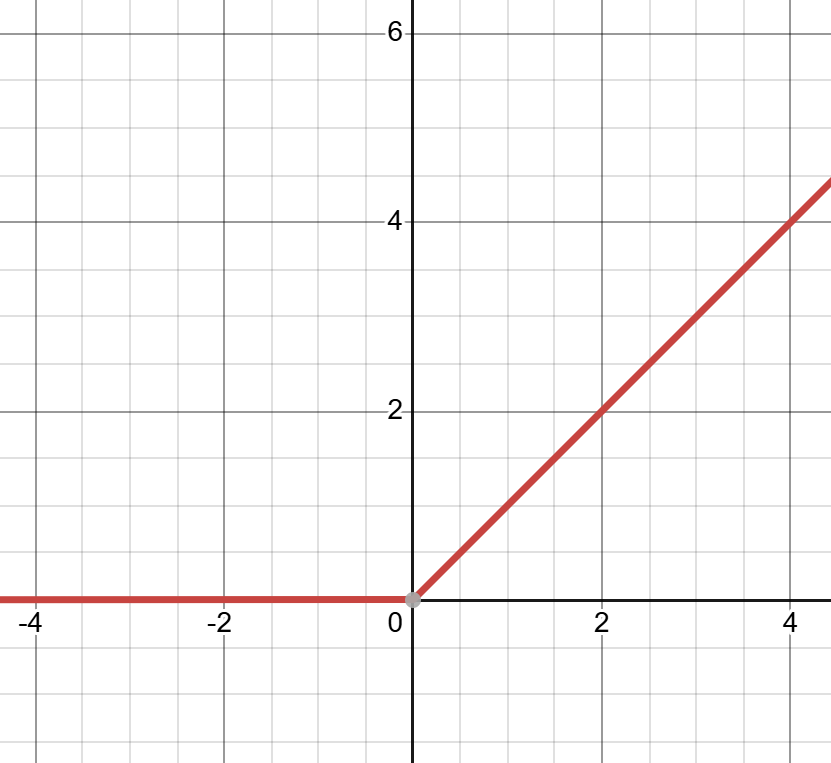
\includegraphics{images/image-0001.png}
\caption{ReLU 函数图像}
\end{figure}

这时候问题来了：

ReLU 看起来只是一种信息损失（把负数全变成0），为什么它能让深度神经网络从一个``傻傻的''线性网络，变成拥有各种强大功能的网络呢？

答案正是：非线性 (Non-linearity) 。

这个``拦住负数''的简单动作，引入了一个``折痕''或``关节''。想象一根直木棍（线性函数）。各种直线加加减减乘系数，得到的显然还是直线。但如果有了``关节''（ReLU函数），情况就完全不同了。

我们现在有四个线性函数：

\begin{figure}[htbp]
\centering
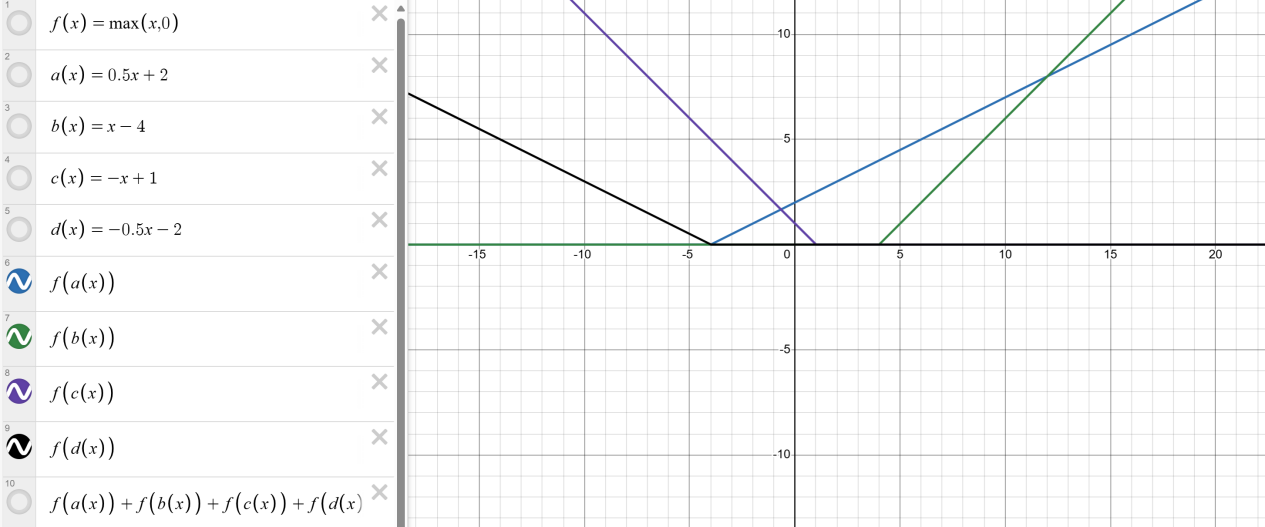
\includegraphics{images/image-0002.png}
\caption{ReLU 变换前的线性函数}
\end{figure}

分别经过ReLU函数（图中用f表示）后如下，可以发现每个函数经过ReLU函数时的``关节位置''和``伸展方向''不同：

\begin{figure}[htbp]
\centering
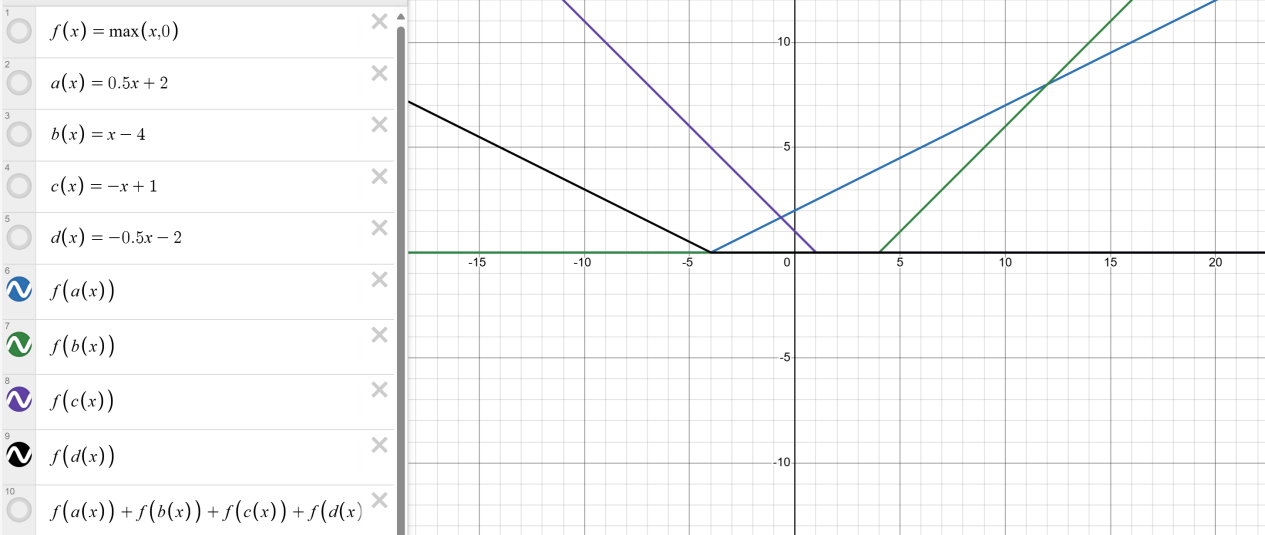
\includegraphics{images/image-0003.png}
\caption{ReLU 变换后的分段线性函数}
\end{figure}

再相加，每一个不同的``关节''都成为了新函数的``关节''：

\begin{figure}[htbp]
\centering
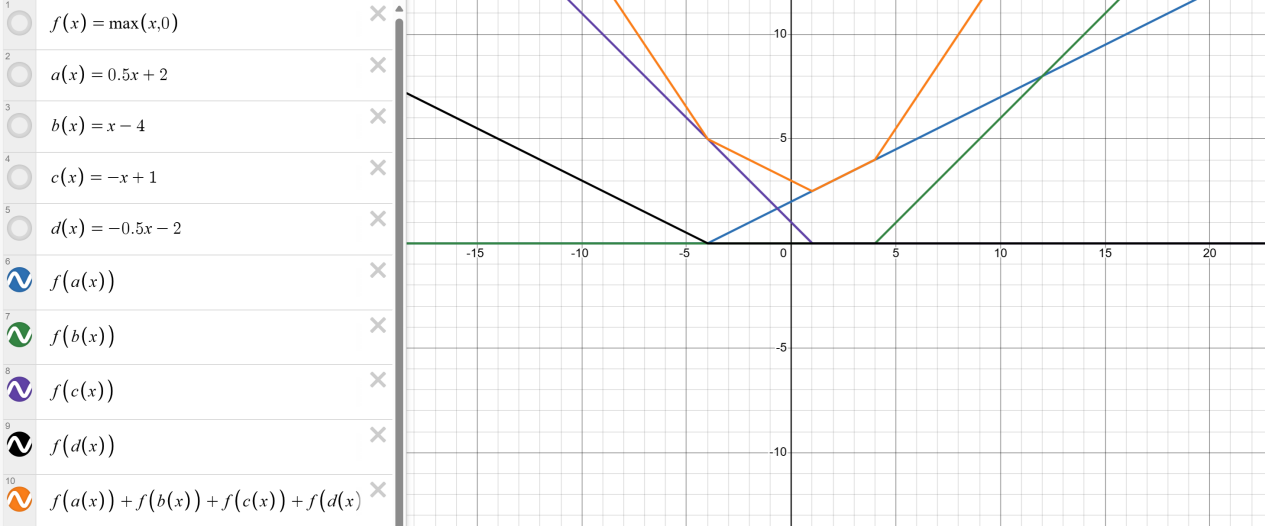
\includegraphics{images/image-0004.png}
\caption{多个 ReLU 函数相加得到更复杂的分段线性函数}
\end{figure}

这就是通用近似定理（Universal Approximation Theorem）的通俗理解：只要你有足够多的带``关节''（非线性激活函数）的神经元，理论上你可以``拼''出（拟合）宇宙中任何一个复杂的函数。

当然，``一刀切''地把负数全砍掉有时太粗暴了。万一负数信息也有用呢？于是研究者们发明了一些变种，比如 Leaky ReLU，它允许负数``泄露''一点点信息过去：f(x) = max(x, 0) + a*min(x, 0)，当a=0时，就变回了普通的ReLU。

\hypertarget{ux56dbux635fux5931ux51fdux6570}{%
\subsection{四、损失函数}\label{ux56dbux635fux5931ux51fdux6570}}

刚才我们搭建了一台由``师傅''（神经元）和``关节''（ReLU）组成的``函数机器''。它现在可以对输入x给出自己的输出y了。那么，我们怎么知道它输出的 \(y\) 是``好''还是``坏''呢？

就像考试需要``评分标准''一样，AI也需要一个``评分标准''来衡量它的预测结果和``标准答案''之间的差距。这个``评分标准''就是损失函数（Loss Function）。损失函数是一个``打分器''。把AI的全部参数丢进去，它会根据输入和输出算出一个损失值（Loss）。训练AI的唯一目标，就是通过不断调整参数，最终寻找到一组参数，让这个``损失值''变得最小，也就是它的输出最接近我们期望达到的目标，完美预测时的损失为0。在线性回归中，这组参数是可以算出解析解的，但在大部分问题中并不能（后续会讲优化参数的方法）。

回归问题中，最常用的损失函数是平方误差函数。当样本的预测值为 \(\hat{y}\)，其相应的真实标签为 \(y\) 时，平方误差可以定义为：

\[
Loss=\frac{1}{2}(\hat{y}-y)^2
\]

对于一个批量的 \(n\) 个样本，总损失为：

\[
Loss=\frac{1}{2}\sum_{i=1}^{n}(\hat{y}_i-y_i)^2
\]

这实际上就是最小二乘法。（常数不同没有本质差别，取1/2是为了让损失函数求导后常数系数为1，在后续计算梯度时更加方便）

高中课本告诉我们均方损失是因为绝对值函数没有那么良好的性质。但是我们为什么偏偏选择``平方''呢？

一方面，前面已经阐述过，它求导会得到 \(\hat{y}-y\) 这个简洁的项，可以让后续求解梯度更加方便。但是其实，均方损失的背后还有深刻的统计学含义。

我们假设AI的预测是准的，但现实中总会有一些随机的误差（也就是``噪声''），使得数据集中的数据并不完全符合它本应该符合的函数分布。我们假设这些``噪声''服从高斯分布（正态分布）。假设这个完全正确的AI的参数为θ，此时根据公式，输入x的时候，输出y的概率密度（在输出值连续的情况下，可以理解为输出值介于y和y+dy之间的概率除以dy）为：

\[
p(y \mid \mathbf{x};\theta)=\frac{1}{\sqrt{2\pi\sigma^2}}\exp\left(-\frac{(y-f(\mathbf{x};\theta))^2}{2\sigma^2}\right).
\]

我们希望这个概率越大越好，这就是``极大似然估计''，这里σ是高斯分布的系数。为了让这个概率最大，只需要让指数里的那个括号里的项最小，那一项正是参数为θ下的均方损失。

后续，我们还会介绍另一种损失函数------交叉熵损失函数。

\hypertarget{ux53c2ux8003ux6587ux732e}{%
\subsection{参考文献}\label{ux53c2ux8003ux6587ux732e}}

\begin{itemize}
\tightlist
\item
  Goodfellow, I., Bengio, Y., \& Courville, A. (2016). \href{https://www.deeplearningbook.org/}{Deep Learning}. MIT Press.
\item
  Cybenko, G. (1989). \href{https://doi.org/10.1007/BF02551274}{Approximation by superpositions of a sigmoidal function}. Mathematics of Control, Signals and Systems, 2, 303-314.
\item
  Glorot, X., Bordes, A., \& Bengio, Y. (2011). \href{https://proceedings.mlr.press/v15/glorot11a.html}{Deep Sparse Rectifier Neural Networks}. AISTATS 2011.
\end{itemize}

\clearpage

\hypertarget{ux68afux5ea6ux4e0bux964dux4e0eux53cdux5411ux4f20ux64ad}{%
\section{梯度下降与反向传播}\label{ux68afux5ea6ux4e0bux964dux4e0eux53cdux5411ux4f20ux64ad}}

\hypertarget{ux4e00ux68afux5ea6ux4e0bux964d}{%
\subsection{一、梯度下降}\label{ux4e00ux68afux5ea6ux4e0bux964d}}

\begin{enumerate}
\def\labelenumi{\arabic{enumi}.}
\tightlist
\item
  基本原理
\end{enumerate}

我们现在有了一台``机器''（神经网络），也知道如何给它``打分''（损失函数）。接下来的问题是：AI如何根据这个``分数''来``自我改进''呢？

想象一下，你（AI）站在一个n+1维的巨大山脉（``损失关于n维参数的曲面''）上，山上全是浓雾（全局函数无法直接求解得出）。你的目标是找到海拔最低的``山谷''（Loss最小值）。你看不见谷底在哪，只能往``下降最快''的方向走。

在数学上，梯度（Gradient）是一个向量，它的每一个值代表因变量（Loss）对每个自变量的偏导数值（可以理解为其他变量不变时，因变量对该自变量的导数，即因变量变化量/该自变量变化量的极限）：

\[
\nabla L = \left(\frac{\partial L}{\partial \theta_1}, \frac{\partial L}{\partial \theta_2}, \ldots, \frac{\partial L}{\partial \theta_n}\right)
\]

梯度指示的是参数发生改变时损失的增加量，而我们希望损失下降，所以会在梯度向量前面加一个负号，取它的反方向。对于一个有n个参数的模型，负梯度向量是一个集合了``n个方向陡峭程度''的``指令包''。如第一项代表``只改变θ1时，海拔（L）下降的快慢'' 。

\begin{figure}[htbp]
\centering
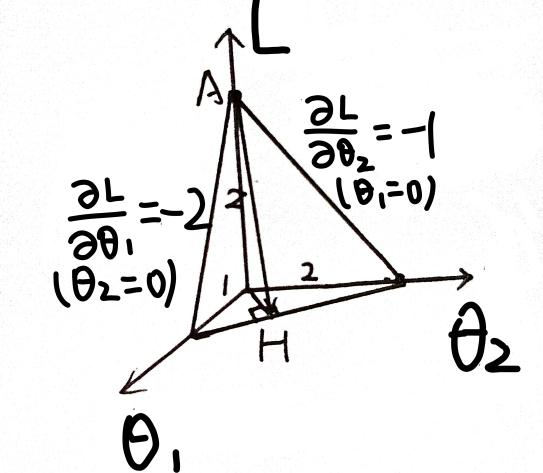
\includegraphics{images/image-0005.jpeg}
\caption{梯度下降方向示意图}
\end{figure}

比如上图中，只有两个参数，损失L是一个由两个输入决定的函数。损失L在θ1方向的``陡峭度''是-1，θ2方向的``陡峭度''是-2，负梯度向量就是(1, 2)。而``下降最快''的路径AH在参数空间（也就是图中的底面）上的投影OH（即``等高线最密集''的方向）的方向和负梯度向量(1, 2)相同。这也就说明了我们应该沿着负梯度方向下降。

\begin{enumerate}
\def\labelenumi{\arabic{enumi}.}
\setcounter{enumi}{1}
\tightlist
\item
  学习率调节
\end{enumerate}

我们知道了梯度改变的方向，那么改变多少呢？

一般我们会把负梯度向量乘以一个常数，它称为学习率。这个学习率是一个超参数，它自身无法通过梯度下降法来优化，只能人为调整好。下面两张图是从L轴看，如果学习率过大或过小，参数更新时会出现的问题。如果学习率太大，可能会出现``震荡''的情形，始终无法取到最低点，甚至适得其反；如果学习率太小，会导致步长太小，梯度下降需要的步数更多，计算量和计算开销更大。

\begin{figure}[htbp]
\centering
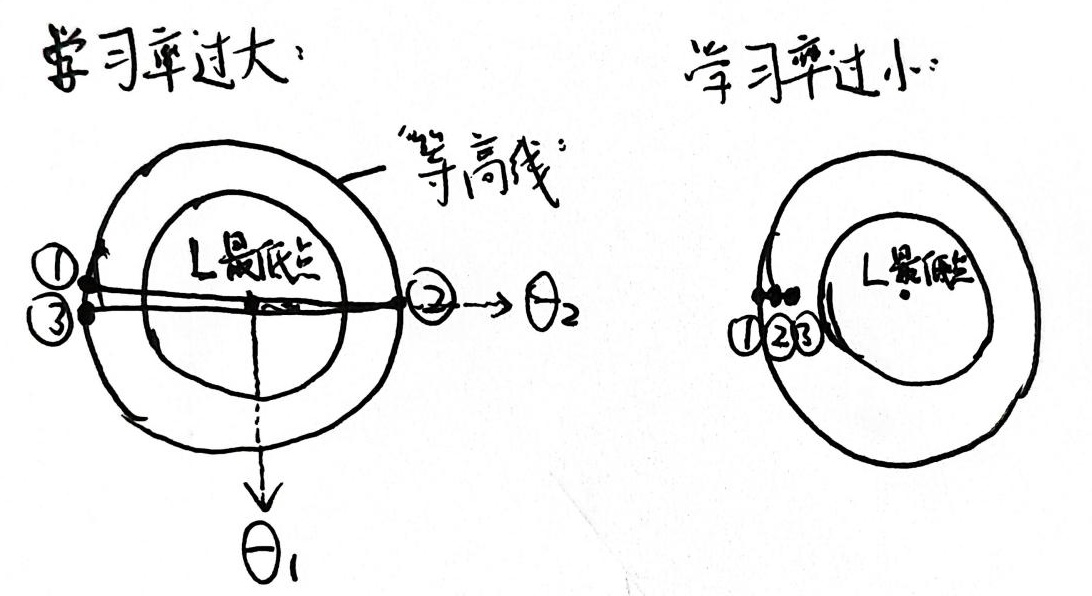
\includegraphics{images/image-0006.jpeg}
\caption{学习率过大或过小的影响}
\end{figure}

\begin{enumerate}
\def\labelenumi{\arabic{enumi}.}
\setcounter{enumi}{2}
\tightlist
\item
  小批量随机梯度下降
\end{enumerate}

我们知道了梯度下降，但是这里的Loss应该取谁的损失呢？

如果取所有样本的平均，不仅计算开销大，而且因为每一步取的都是相同样本的Loss对参数的函数，缺乏随机性，很容易``陷入''局部最小值，``出不来了''；如果只取一个样本，又随机性太大。因此，我们一般会把样本随机分为多个小批量（Mini-Batch），每次利用一个批量的数据计算Loss对各个参数的负梯度，进行梯度下降，这样就兼顾了准确性、适当的随机性和计算开销。

\hypertarget{ux4e8cux53cdux5411ux4f20ux64ad}{%
\subsection{二、反向传播}\label{ux4e8cux53cdux5411ux4f20ux64ad}}

我们已经知道，AI需要沿着负梯度方向这个``指令包''来下山。但一个关键问题悬而未决：在一个拥有数百万甚至数十亿参数的复杂神经网络中，如何高效地计算出这个包含损失函数对所有参数的梯度（即每个方向的``陡峭度''）的``指令包''呢？

反向传播是一种利用链式法则，从输出层开始，逐层向后（反向）计算损失函数对网络中每一个参数的偏导数的算法。我们可以把它理解为一个精妙的责任与误差分配系统。

\begin{enumerate}
\def\labelenumi{\arabic{enumi}.}
\tightlist
\item
  一个直观的比喻：生产线与责任追溯
\end{enumerate}

想象一个生产巧克力的工厂（神经网络）：输入可可粉、糖、牛奶等原材料（输入数据），经过混合、加热、搅拌、冷却、塑形等多层工序（网络层），输出一块成品巧克力（预测结果），质检品尝后给出评分，比如``太苦了''（计算损失）。现在发现巧克力太苦（损失很大），工厂需要改进。反向传播要解决的问题是：如何精确地知道每一道工序应该承担多少``责任''？是搅拌工序（某一中间层）没搅匀吗？还是加热工序（另一层）温度不对？或者说，根本就是采购的可可粉（输入数据）本身浓度太高？

它会进行精准的责任追溯：

质检员（损失函数）~首先确定最终产品``苦''的程度（损失L输出的梯度），回溯给最后的塑形工序：``你的产品太苦了，偏差量为xxx。''塑形工序收到反馈后想：``我本身只是塑形，苦味主要来自冷却工序传给我的半成品，而且根据我的工艺（激活函数），我对苦味的敏感度是这样的\ldots{}'' 于是它结合自己的``工艺特性''（本地梯度），计算出了对上一道工序（冷却工序）的责任指控，并把这个指控向后传递。这个过程逐层反向进行，每一层都根据后一层传来的``指控''和自身的``工艺说明书''（本地函数和其导数），计算出自己对问题的责任，并继续向更前端的工序追溯。最终，这个误差信号被传递到了最开始的原材料采购（输入层）~和每一道具体的工序。于是，每个环节都清楚地知道了：``哦，我需要为这个`苦'的结果负XX\%的责任。''

\begin{enumerate}
\def\labelenumi{\arabic{enumi}.}
\setcounter{enumi}{1}
\tightlist
\item
  数学表达
\end{enumerate}

这个``责任追溯''在数学上是通过微积分中的链式法则实现的。链式法则用于计算复合函数的导数。

假设一个简单的网络：输入层x -\textgreater{} 中间层h = f(w1\emph{x) -\textgreater{} 输出层y = g(w2}h) -\textgreater{} 损失L(y)

我们想求损失L关于第一个参数w1的梯度。根据链式法则：

\[
\frac{\partial L}{\partial w_1}=\frac{\partial L}{\partial y}\cdot\frac{\partial y}{\partial h}\cdot\frac{\partial h}{\partial w_1}
\]

反向传播的过程就是从上式右边向左计算：

\begin{enumerate}
\def\labelenumi{\arabic{enumi}.}
\tightlist
\item
  前向传播：先进行一次完整的从x到L的计算，记录下每一层的中间结果（h，y）。
\item
  反向计算：

  \begin{enumerate}
  \def\labelenumii{\alph{enumii}.}
  \tightlist
  \item
    首先计算 \(\frac{\partial L}{\partial y}\)（损失对输出的梯度）。
  \item
    然后，将这个梯度乘以 \(\frac{\partial y}{\partial h}\)（输出对中间层的梯度），得到 \(\frac{\partial L}{\partial h}\)（损失对中间层的梯度）。这就是将误差从输出层y传递到了中间层h。
  \item
    接着，将 \(\frac{\partial L}{\partial h}\) 乘以 \(\frac{\partial h}{\partial w_1}\)（中间层对参数w1的梯度），最终得到我们想要的 \(\frac{\partial L}{\partial w_1}\)。
    同理，L对w2的梯度也就是L对y的梯度乘以y对w2的梯度.计算出L对所有层的梯度后， 执行梯度下降即可。
  \end{enumerate}
\end{enumerate}

\hypertarget{ux4e09ux68afux5ea6ux6d88ux5931ux548cux68afux5ea6ux7206ux70b8}{%
\subsection{三、梯度消失和梯度爆炸}\label{ux4e09ux68afux5ea6ux6d88ux5931ux548cux68afux5ea6ux7206ux70b8}}

\hypertarget{ux4e00ux539fux56e0}{%
\subsubsection{（一）原因}\label{ux4e00ux539fux56e0}}

在反向传播中，为了计算靠近输入层的参数的梯度，我们需要将后面所有层的梯度连乘起来。对于一个L层的网络，损失对第一层权重 \(W^{[1]}\) 的梯度：

\[
\begin{aligned}
\frac{\partial L}{\partial W^{[1]}}
&=
\frac{\partial L}{\partial a^{[L]}}
\cdot
\frac{\partial a^{[L]}}{\partial z^{[L]}}
\cdot
\frac{\partial z^{[L]}}{\partial a^{[L-1]}} \\
&\quad \cdots
\cdot
\frac{\partial a^{[2]}}{\partial z^{[2]}}
\cdot
\frac{\partial z^{[2]}}{\partial a^{[1]}}
\cdot
\frac{\partial a^{[1]}}{\partial z^{[1]}}
\cdot
\frac{\partial z^{[1]}}{\partial W^{[1]}} .
\end{aligned}
\]

在深层网络中，如果其中大部分项的绝对值~小于1，那么连乘的结果会指数级地趋近于0，导致参数更新的幅度变得极小，网络的前面层几乎停止学习，参数更新微不足道。深度网络退化为一个只有后面几层在学习的浅层网络，无法发挥深度模型的表征能力。训练过程变得极其缓慢，甚至完全停滞。

反之，如果大部分项的绝对值~大于1，结果则会指数级地增长到无穷大，导致权重更新的幅度变得极大。参数更新步长巨大且不稳定，导致损失函数剧烈震荡，无法收敛。模型参数可能变成NaN（非数字），因为更新的值超出了计算机的浮点数表示范围。模型完全无法学习到有意义的模式。

\hypertarget{ux4e8cux89e3ux51b3ux65b9ux6848}{%
\subsubsection{（二）解决方案}\label{ux4e8cux89e3ux51b3ux65b9ux6848}}

\begin{enumerate}
\def\labelenumi{\arabic{enumi}.}
\item
  激活函数选择：使用x＞0时导数恒为1的ReLU函数，而不是在x很大或很小时导数趋于0的Sigmoid函数。
\item
  参数初始化技巧：后续会介绍。
\item
  批量规范化：强制将每一层的输入拉回到标准正态分布，以让该层最终整体的梯度尽量接近1。
\item
  模型架构设计：如ResNet，通过``输出=x+f(x)''的设计（x为输入，f为模型层），建立一条从输入x``直达''输出的``梯度高速公路''，让梯度可以无损地直接流向较浅的层，从根本上解决了深层网络（如上百层的 ResNet）的梯度消失问题。
\item
  梯度裁剪：针对梯度爆炸，可以在更新权重前，检查梯度的范数（梯度向量的长度）。如果超过设定的阈值，就对梯度在各个方向进行等比例缩放，使其范数（长度）在阈值以内：
\end{enumerate}

如果 \(\lVert g\rVert > \text{threshold}\)，则：

\[
g\leftarrow \frac{\text{threshold}}{\lVert g\rVert}\cdot g
\]

\hypertarget{ux53c2ux8003ux6587ux732e-1}{%
\subsection{参考文献}\label{ux53c2ux8003ux6587ux732e-1}}

\begin{itemize}
\tightlist
\item
  Rumelhart, D. E., Hinton, G. E., \& Williams, R. J. (1986). \href{https://doi.org/10.1038/323533a0}{Learning representations by back-propagating errors}. Nature.
\end{itemize}

\clearpage

\hypertarget{ux8fc7ux62dfux5408}{%
\section{过拟合}\label{ux8fc7ux62dfux5408}}

\hypertarget{ux4e00ux8fc7ux62dfux5408ux4e0eux6b20ux62dfux5408}{%
\subsection{一、过拟合与欠拟合}\label{ux4e00ux8fc7ux62dfux5408ux4e0eux6b20ux62dfux5408}}

在训练时，我们只能看到模型在训练集上的Loss，我们希望它变小。但是这是可以``作弊''的：如果模型单纯``记住''所有数据，它的训练Loss为零，但在真实世界中毫无用处。比如一个医疗模型，部署时模型需要判断从未见过的患者。只有当模型真正发现了一种泛化模式时，才会作出有效的预测。我们如何才能确定模型是真正发现了一种泛化的规律，而不是简单地记住了数据呢？

\begin{enumerate}
\def\labelenumi{\arabic{enumi}.}
\tightlist
\item
  训练误差和泛化误差
\end{enumerate}

训练误差（Training Error）：模型在训练数据集上计算得到的误差。

泛化误差（Generalization Error）：模型应用在同样从原始样本的分布中抽取的无限多数据样本时，模型误差的期望。

困难在于，泛化误差是一个理想化的数值，我们永远无法准确计算（因为我们无法获取无限的数据）。在实际中，我们只能通过将模型应用于一个独立的测试集来估计泛化误差。

\begin{enumerate}
\def\labelenumi{\arabic{enumi}.}
\setcounter{enumi}{1}
\tightlist
\item
  过拟合
\end{enumerate}

所谓``过拟合''，就是训练误差很低，但泛化误差很高的情况。

过拟合可以用大家熟悉的一个例子来解释：大家在备战高考的时候，在模拟考试里取得好成绩并不能保证在高考时考好。例如，模拟考试经常一味模仿上一年的高考题，如果学生就把这种题目的套路和手法做得很熟，却会在面对高考的新题时无所适从，这就是``过拟合''。备战高考的学生在做模拟题时，只有理解和掌握其背后可迁移的普遍思想方法，才能在面对高考的新题时游刃有余；同样的，对于模型而言，只有学习到数据背后的泛化规律，才能进行有效的预测。

再比如一个小学生，如果理解了公式原理（如1+1=2），即使考试题目将数字从1换成了5，他依然能计算出正确答案。这意味着他的``泛化误差''很低。过拟合的学习则像一个记忆力超群的学生，把练习册上每一道题的答案都背了下来，在平时练习里能拿满分（训练误差为 0），到了期末考试，题目稍微变动一点，出现一个他没见过的数字（比如9），他就完全不会了。

\begin{enumerate}
\def\labelenumi{\arabic{enumi}.}
\setcounter{enumi}{2}
\tightlist
\item
  过拟合与模型复杂度的关系
\end{enumerate}

模型复杂性由什么构成是一个复杂的问题。通常对于神经网络，参数越多、取值范围越大、训练时间越长，模型就越复杂。为了直观地解释``模型复杂性''如何导致过拟合，我们来看一个经典的多项式拟合例子。

假设真实世界的数据规律是一个简单的二次函数（抛物线），再加上一点点观测时的随机误差（噪声）：y=ax\^{}2+bx+c+epsilon。如果我们使用一个过于复杂的模型，比如一个9次多项式y = w\_9x\^{}9 + w\_8x\^{}8 + \ldots{} + w\_1x + w\_0（拥有10个参数）来拟合这些数据，因为模型有10个自由度，它有足够的能力去扭曲自己，好比我们允许模型使用一把极度柔软、可以随意弯曲的尺子去连接纸上的点，它会强行穿过每一个因为测量误差而偏离真实轨迹的样本点。

为了穿过那些不规则分布的噪声点，模型被迫让高次项的系数（如w\_9）变得非常大。对于高次项x\^{}9，输入x只要有极其微小的变化，输出值y就会发生巨大的爆炸式变化。最终拟合出来的函数曲线不再是一条平滑的抛物线，而变成了一条上下翻飞、剧烈震荡的``心电图''。虽然它完美穿过了所有训练点，但在测试点上，这种剧烈的震荡会导致预测值非常离谱（9次函数和2次函数随机取点相差大概率是非常大的）。

而欠拟合则相反，如用一条直线拟合二次函数，模型灵活度太低，无法把握数据间的规律，效果不好。

\hypertarget{ux4e8cux589eux52a0ux8badux7ec3ux6570ux636eux91cf}{%
\subsection{二、增加训练数据量}\label{ux4e8cux589eux52a0ux8badux7ec3ux6570ux636eux91cf}}

过拟合意味着模型复杂度显著大于数据量。对于相同的模型，训练数据集中的样本越少，我们就越有可能（且更严重地）过拟合；对于相同量的数据，模型复杂度越大，越可能过拟合。因此，我们可以增大训练数据量，或降低模型复杂度。这里探讨增大数据量。

这里涉及到一个核心假设：独立同分布假设。我们假设训练数据和测试数据都是从相同的概率分布中独立提取的。如果数据分布发生变化（例如，用大学生的照片训练人脸识别，去识别养老院的老人），模型就会失效。

即便分布一致，如果数据量太少（例如只有几千张图片），复杂的深度学习模型很容易就能``记住''所有图片，而不是学习特征。深度学习目前的繁荣，很大程度上归功于海量数据集的出现，使得我们能够训练复杂的模型而不过度过拟合。

在垂直任务中，我们的真实数据往往非常少或非常昂贵。如在医学影像（如CT或MRI）中，要诊断一种罕见的癌症。我们可能只有几百张（甚至几十张）带标签的``阳性''图像。此时为了解决过拟合，可以进行以下处理：

\begin{enumerate}
\def\labelenumi{\arabic{enumi}.}
\item
  迁移学习：利用已经在大数据集上预训练好的大模型，在这些小型数据集上进行微调。
\item
  对已有数据进行变换：对于图像而言，就是旋转、裁剪、缩放、翻转、平移、添加噪声、改变对比度或亮度等。
\item
  利用VAE（变分自编码器）：在编码-解码的过程中，一个 VAE 的编码器输出一个概率分布，解码器不是从一个``点''来重建，而是从这个``模糊区域''中随机采样一个点来进行重建。
\item
  利用GAN生成：我们可以训练一个基于生成器-判别器架构的GANs模型（比如一个变种的DCGAN或WGAN），判别器以这几百张真实癌症图像的分布为参考基准。一旦训练完成，这个GANs的生成器就可以从随机噪声开始，生成成千上万张看起来逼真、但又与原始图像不完全相同的``假''癌症图像。
\end{enumerate}

\hypertarget{ux4e09ux6a21ux578bux6b63ux5219ux5316ux964dux4f4eux6a21ux578bux590dux6742ux5ea6ux89c1ux540eux7eedux5173ux4e8eux6a21ux578bux6b63ux5219ux5316ux7684ux5185ux5bb9}{%
\subsection{三、模型正则化（降低模型复杂度，见后续关于模型正则化的内容）}\label{ux4e09ux6a21ux578bux6b63ux5219ux5316ux964dux4f4eux6a21ux578bux590dux6742ux5ea6ux89c1ux540eux7eedux5173ux4e8eux6a21ux578bux6b63ux5219ux5316ux7684ux5185ux5bb9}}

\hypertarget{ux53c2ux8003ux6587ux732e-2}{%
\subsection{参考文献}\label{ux53c2ux8003ux6587ux732e-2}}

\begin{itemize}
\tightlist
\item
  Aston Zhang, Zachary C. Lipton, Mu Li, Alexander J. Smola. (2023). \href{https://zh.d2l.ai/}{《动手学深度学习》}. Cambridge University Press.
\end{itemize}

\clearpage

\hypertarget{ux4ea4ux53c9ux71b5ux635fux5931ceux4e0esoftmaxux56deux5f52}{%
\section{交叉熵损失（CE）与Softmax回归}\label{ux4ea4ux53c9ux71b5ux635fux5931ceux4e0esoftmaxux56deux5f52}}

\hypertarget{ux4e00ux4ea4ux53c9ux71b5ux635fux5931ux51fdux6570cross-entropyce}{%
\subsection{一、交叉熵损失函数（Cross Entropy,CE）}\label{ux4e00ux4ea4ux53c9ux71b5ux635fux5931ux51fdux6570cross-entropyce}}

在分类任务中，例如要看一张图，判断它是``猫''、``狗''还是``鸟''。AI会给出一个``概率分布''，比如q={[}猫: 0.7, 狗: 0.2, 鸟: 0.1{]}，标准答案： 真实答案也是一个概率分布，p={[}猫: 1, 狗: 0, 鸟: 0{]}。这时用MSE来量q\_i和p\_i之间的``距离''就非常不合适了。下面我们引入信息论中的``信息熵''和``交叉熵''概念。

信息论认为，信息是用来消除随机不确定性的东西。信息量取决于不确定性，它可以被理解为一种``惊讶度''，或者说描述这个事件发生的所有可能性所需要的编码数：

如果一个事件必然发生（概率~P=1），它不需要任何编码信息，你已经知道了它必然发生，因此毫不惊讶，惊讶度为~-log₂(1) = 0比特。

如果一个事件有25\%的概率发生（P=0.5），这个事件的可能性等同于在00、01、10、11四个2位数编码中随机选择一个，在事件最终发生的那一刻，你获得了2比特的信息，有一些惊讶，惊讶度是~-log₂(0.25) = 2比特。

如果一个事件非常罕见（概率~P -\textgreater{} 0），惊讶度趋近于无穷大。在事件最终发生的那一刻，你极度惊讶。

对于一个离散的概率分布P，假设共有n种可能发生的事件，概率分别为(i=1,\ldots,n)，则信息量，或者说应该分配的编码数的期望为.

在机器学习中，我们有一个真实的分布~P（数据的真实标签），和一个模型预测的分布~Q。我们想知道这两个分布之间有多``不同''。KL散度，也称为相对熵，就是用来衡量用一个近似分布~Q去描述真实分布~P时，所产生的信息损耗。

从P到Q的KL散度定义为：

\[
D_{\mathrm{KL}}(P \parallel Q)=\sum_i p(i)\log\left(\frac{p(i)}{q(i)}\right)
\]

其中表示在真实概率为~p(i)的事件上，用~q(i)来描述它所产生的``信息差异''或``惊讶程度''。KL散度是将所有事件上的这种``信息差异''用真实概率p(i)~进行加权平均，是一个恒非负的函数，当且仅当P、Q两分布完全相同时值为0。

进一步地：

\[
\begin{aligned}
D_{\mathrm{KL}}(P \parallel Q)
&=\sum_i p(i)\log p(i)-\sum_i p(i)\log q(i)\\
&=H(P,Q)-H(P)
\end{aligned}
\]

H(P)是真实分布的信息熵，在分类任务中不变。H(P,Q)就是交叉熵，定义为：

\[
H(P,Q)=-\sum_i p(i)\log q(i)
\]

由于我们的目标是最小化 \(D_{\mathrm{KL}}(P\parallel Q)\)，而 \(D_{\mathrm{KL}}(P\parallel Q)=H(P,Q)-\mathcjk{常数}\)，那么：

\[
\min D_{\mathrm{KL}}(P\parallel Q)\Longleftrightarrow \min H(P,Q)
\]

在监督学习中，真实分布P是确定的值（有真实标签），与模型参数也无关。此时，用交叉熵来代替KL散度在代码上更简洁且不易出现log0错误。

从编码的角度，我们可以把交叉熵损失函数理解为是在用估计的概率分布进行编码，而事件服从真实分布，此时所需的平均编码数期望。

对于分类任务，为0或1（且只有一个值为1），且等于对应的标签值0或1，因此交叉熵损失可以写成为1时，若趋于0，快速增长，相当于只关心应该分入的那一类算出的概率值和1的接近程度（也就是那个，表示应该分入的那一类算出的概率值），不关心其他类。

对于一个批量的样本（如LLM一次性生成n个token），交叉熵损失函数取n个样本的均值.它可以被视为表达n个样本的``平均信息量''。进一步拓展：交叉熵损失函数取指数后，就可以视为整个序列的困惑度（``生成该序列时，每次平均从几个token里选一个''）。困惑度的n次方的倒数就是生成该序列的联合概率。

那么，为什么不使用均方损失呢？

\begin{enumerate}
\def\labelenumi{\arabic{enumi}.}
\item
  理论不符： MSE 衡量的是两个数值向量之间的欧氏距离。而交叉熵衡量的是两个概率分布之间的信息论距离。分类任务的本质是拟合概率分布，而非拟合特定数值。
\item
  梯度消失：以二分类（Sigmoid）为例：当我们计算交叉熵损失函数对分类常用的 Sigmoid 激活函数输入z的梯度时，推导结果极其优美：
\end{enumerate}

\[
\frac{\partial L_{\mathrm{BCE}}}{\partial z}=\hat{y}-y
\]

梯度大小正比于预测值与真实值之间的误差，误差越大，梯度更新越快，这是合理的。但如果使用MSE：

\[
\frac{\partial L_{\mathrm{MSE}}}{\partial z}=(\hat{y}-y)\cdot\sigma'(z)
\]

其中：

\[
\sigma'(z)=\sigma(z)(1-\sigma(z))=\hat{y}(1-\hat{y})
\]

梯度中多了一项 sigma'(z)。当 Sigmoid 函数的输出y\_hat趋近于0或1时，sigma'(z)这一项会趋近于0。 灾难在于：当模型非常自信地预测错误时（例如y\_hat=0.01），sigma'(z)几乎为0，模型明明错得离谱，却无法快速学习（梯度消失），导致训练极其缓慢或卡在局部最优。

\hypertarget{ux4e8csoftmaxux56deux5f52}{%
\subsection{二、Softmax回归}\label{ux4e8csoftmaxux56deux5f52}}

例如多分类问题，需要输出n个可能类别分别的概率，故要把原来该神经元输出的在实数范围内的logits值（如zi）变为e\textsuperscript{zi/(e}z1+\ldots+e\^{}zn)才能作为概率。好处：突出最高值，符合分类问题特性；归一化为0到1之间概率。运用交叉熵损失时：

由于 softmax 和相关的损失函数很常见，因此我们需要更好地理解它的计算方式。将 \(l(\mathbf{y},\hat{\mathbf{y}})\) 代入损失函数，利用 softmax 的定义，可以得到：

\[
\begin{aligned}
l(\mathbf{y},\hat{\mathbf{y}})
&=-\sum_{j=1}^{q}y_j\log\frac{\exp(o_j)}{\sum_{k=1}^{q}\exp(o_k)}\\
&=\sum_{j=1}^{q}y_j\log\sum_{k=1}^{q}\exp(o_k)-\sum_{j=1}^{q}y_jo_j\\
&=\log\sum_{k=1}^{q}\exp(o_k)-\sum_{j=1}^{q}y_jo_j
\end{aligned}
\]

考虑相对于任何未规范化预测 \(o_j\) 的导数，可以得到：

\[
\partial_{o_j}l(\mathbf{y},\hat{\mathbf{y}})
=\frac{\exp(o_j)}{\sum_{k=1}^{q}\exp(o_k)}-y_j
=\mathrm{softmax}(\mathbf{o})_j-y_j
\]

换句话说，导数是 softmax 模型分配的概率与实际发生情况（由独热标签向量表示）之间的差异。

也就是说，在各个方向上的梯度（下降速率）的比值就是每个方向预测值和实际值之差的比值，如模型预测概率{[}0.1, 0.7, 0.2{]}~，真实标签{[}0, 1, 0{]}~，计算出的梯度就是{[}0.1-0, 0.7-1, 0.2-0{]}。均方损失（对应噪声满足高斯分布）也满足这一特点。

实际计算时：

回想一下，softmax 函数为：

\[
\hat{y}_j=\frac{\exp(o_j)}{\sum_k\exp(o_k)}
\]

其中 \(\hat{y}_j\) 是预测的概率分布，\(o_j\) 是未规范化预测 \(\mathbf{o}\) 的第 \(j\) 个元素。如果 \(o_k\) 中的一些数值非常大，那么 \(\exp(o_k)\) 可能大于数据类型允许的最大数字，即上溢（overflow）。为避免这个问题，可以在继续 softmax 计算之前，先从所有 \(o_k\) 中减去 \(\max(o_k)\)。每个 \(o_k\) 按常数移动不会改变 softmax 的返回值：

\[
\begin{aligned}
\hat{y}_j
&=\frac{\exp(o_j-\max(o_k))\exp(\max(o_k))}
{\sum_k\exp(o_k-\max(o_k))\exp(\max(o_k))}\\
&=\frac{\exp(o_j-\max(o_k))}
{\sum_k\exp(o_k-\max(o_k))}
\end{aligned}
\]

尽管我们要计算指数函数，但最终在计算交叉熵损失时会取它们的对数。通过将 softmax 和交叉熵结合在一起，可以直接使用 \(o_j-\max(o_k)\)，避免反向传播过程中可能困扰我们的数值稳定性问题：

\[
\begin{aligned}
\log(\hat{y}_j)
&=\log\left(\frac{\exp(o_j-\max(o_k))}
{\sum_k\exp(o_k-\max(o_k))}\right)\\
&=\log(\exp(o_j-\max(o_k)))
-\log\left(\sum_k\exp(o_k-\max(o_k))\right)\\
&=o_j-\max(o_k)-\log\left(\sum_k\exp(o_k-\max(o_k))\right)
\end{aligned}
\]

\hypertarget{ux4e09ux4e8cux5143ux4ea4ux53c9ux71b5ux635fux5931bce}{%
\subsection{三、二元交叉熵损失（BCE）}\label{ux4e09ux4e8cux5143ux4ea4ux53c9ux71b5ux635fux5931bce}}

\begin{enumerate}
\def\labelenumi{\arabic{enumi}.}
\tightlist
\item
  二元交叉熵的数学表达
\end{enumerate}

当分类问题只有两个类别（真或假）可以二选一时，假设为真的实际概率为p，预测为真的概率为q，实际数据标签（真为1，假为0）为y，则真实二元交叉熵的公式为-p\emph{logq-(1-p)}log(1-q)，又y=p，也可写成-y\emph{logq-(1-y)}log(1-q).

\begin{enumerate}
\def\labelenumi{\arabic{enumi}.}
\setcounter{enumi}{1}
\tightlist
\item
  模型给出预测概率q的方式
\end{enumerate}

当只有两个类别时，我们就不再需要输出多个logits值后用Softmax了，而是只需要一个logit，用sigmoid函数得到为其中某一类（如选择``是''）的概率，再用二元交叉熵。事实上可以证明这种操作就是Softmax的一种特殊情况：

对于两个类别，Softmax输出为：

\[
p_0=\frac{e^{z_0}}{e^{z_0}+e^{z_1}},\qquad
p_1=\frac{e^{z_1}}{e^{z_0}+e^{z_1}}
\]

只关心第二个类别的概率 \(p_1\)，并定义 \(z=z_1-z_0\)：

\[
p_1=\frac{e^{z_1}}{e^{z_0}+e^{z_1}}
=\frac{1}{1+e^{-(z_1-z_0)}}
=\sigma(z_1-z_0)
\]

所以二元Softmax可以简化为Sigmoid函数，其中输入是两类logits的差值。

\begin{enumerate}
\def\labelenumi{\arabic{enumi}.}
\setcounter{enumi}{2}
\tightlist
\item
  BCE在多标签分类中的运用
\end{enumerate}

由于Softmax函数只适用于``n选一''式的``单选''分类，如果我们需要同时将一个对象分到多个类别（如给蛋白质加各种功能标签），进行``多选''分类，Softmax就不适用了。这时我们可以把任务看成有很多（样本，类别）组合，对于每一个组合，都分别判断该对象是否分入该类别。此时，交叉熵损失先按所有（样本，类别）组合加起来，然后按组合总数取平均。

多标签交叉熵损失的代码实现：

\begin{verbatim}
import torch

import torch.nn as nn

# 假设批次大小=2，类别数=3

logits = torch.tensor([[1.2, -0.5, 0.8],[-0.3, 1.5, -1.0]]) #模型输出的原始值（未经过激活函数）

targets = torch.tensor([[1, 0, 1], [0, 1, 0]], dtype=torch.float) #真实标签，这里用0和1表示每个样本是否属于某个类别

# 使用BCEWithLogitsLoss（默认reduction='mean'即取平均模式）

criterion = nn.BCEWithLogitsLoss()

loss = criterion(logits, targets)

print(f"损失值: {loss.item()}")

# 手动验证计算过程

sigmoid_outputs = torch.sigmoid(logits)

bce_per_element = - (targets * torch.log(sigmoid_outputs) +

(1 - targets) * torch.log(1 - sigmoid_outputs)) #相同形状的矩阵，Pytorch执行按元素乘法

print(f"每个(样本,类别)的损失:\n{bce_per_element}")

total_loss = bce_per_element.sum()

num_elements = bce_per_element.numel()  # N × C = 2 × 3 = 6

manual_loss = total_loss / num_elements

print(f"手动计算的平均损失: {manual_loss.item()}")
\end{verbatim}

\hypertarget{ux53c2ux8003ux6587ux732e-3}{%
\subsection{参考文献}\label{ux53c2ux8003ux6587ux732e-3}}

\begin{itemize}
\tightlist
\item
  Aston Zhang, Zachary C. Lipton, Mu Li, Alexander J. Smola. (2023). \href{https://zh.d2l.ai/}{《动手学深度学习》}. Cambridge University Press.
\end{itemize}

\clearpage
